%\begin{name}
%	{Biên soạn đề: Loc Do\\ Phản biện: Nguyễn Văn B}
%	{ĐỀ THI THỬ SỞ NGHỆ AN LẦN 1} 
%\end{name}
\section{Sở GD\&ĐT Nghệ An 25--26, Lần 1}

\caulc
\Opensolutionfile{ans}[ans/ansBONPA-NgheAn-L1]
%%%%%%%%%%%%%%%%%%%%%%%%%%%%%%%%%%%%%%%%%%%%%%%%%%%%%%%%%
\begin{ex}%[1D3N2-2]
	Giá trị của $\lim\limits_{x\to 0}\dfrac{1}{x+1}$ bằng
	\choice
		{$\dfrac{1}{2}$}
		{\True $1$}
		{$+\infty$}
		{$0$}
	\loigiai{
		Ta có $\lim\limits_{x\to 0}\dfrac{1}{x+1} = \dfrac{1}{0+1} = 1$.
	}
\end{ex}

\begin{ex}%[2D1H5-1]
	\immini{Hàm số nào sau đây có đồ thị như hình vẽ?
		\choice [2]
			{$f(x)=x^3+3x+1$}
			{$f(x)=-x^3+3x-1$}
			{\True $f(x)=-x^3+3x+1$}
			{$f(x)=x^3-3x-1$}}{
		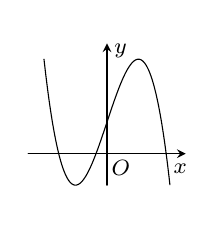
\begin{tikzpicture}[scale=.4, font=\footnotesize, line join=round, line cap=round, >=stealth]
    \draw[->] (-2.5,0)--(2.5,0) node[shift={(-110:0.2)}] {$x$};
			\draw[->] (0,-1)--(0,3.5) node[shift={(-30:0.2)}] {$y$};
			\clip (-2.5,-2) rectangle (2.5,4);
			\draw[smooth,samples=100,domain=-2:2] plot(\x,{-(\x)^3+3*\x+1});
			\foreach \x/\y/\ang/\dist/\lbl in {0/0/-45/0.25/O} \fill (\x,\y) circle (1pt) node[shift={(\ang:\dist)}] {$\lbl$};
    \end{tikzpicture}
		}
	\loigiai{
		Từ đồ thị, ta thấy $\lim\limits_{x\to +\infty} f(x) = -\infty$ nên hệ số $a < 0$, do đó loại phương án $f(x)=x^3+3x+1$ và $f(x)=x^3-3x-1$.\\
		Đồ thị hàm số cắt trục tung tại điểm có tung độ dương nên $f(0) > 0$, do đó loại phương án $f(x)=-x^3+3x-1$.\\
		Vậy hàm số cần tìm là $f(x)=-x^3+3x+1$.
	}
\end{ex}

\begin{ex}%[2D3N1-2]
	Thống kê điểm thi tốt nghiệp môn Toán THPT năm $2024$ của lớp 12D tại một trường THPT thu được kết quả như sau:
	\begin{center}
		\begin{tabular}{|c|c|c|c|c|c|c|c|}
			\hline
			Nhóm & $[3;4)$ & $[4;5)$ & $[5;6)$ & $[6;7)$ & $[7;8)$ & $[8;9)$ & $[9;10]$ \\
			\hline
			Tần số & $3$ & $4$ & $5$ & $10$ & $15$ & $10$ & $5$ \\
			\hline
		\end{tabular}
	\end{center}
	Khoảng biến thiên của mẫu số liệu thống kê trên bằng
	\choice
		{$10$}
		{\True $7$}
		{$6$}
		{$8$}
	\loigiai{
		Khoảng biến thiên của mẫu số liệu ghép nhóm trên là $R = 10 - 3 = 7$.
	}
\end{ex}

\begin{ex}%[2H2N2-2]
	Trong không gian với hệ tọa độ $Oxyz$, cho điểm $M(1;2;3)$. Tọa độ hình chiếu vuông góc của điểm $M$ lên trục $Ox$ là
	\choice
		{$(2;0;0)$}
		{$(3;0;0)$}
		{\True $(1;0;0)$}
		{$(1;0;3)$}
	\loigiai{
		Hình chiếu vuông góc của điểm $M(1;2;3)$ lên trục $Ox$ có tọa độ là $(1;0;0)$.
	}
\end{ex}

\begin{ex}%[2D1N2-2]
	Cho hàm số $y=f(x)$ có bảng biến thiên như sau:
	\begin{center}
		
\begin{tikzpicture}
    \tkzTabInit[nocadre=true, lgt=1, espcl=3, deltacl=0.5] {$x$/0.7,$y'$/0.7,$y$/2} {$-\infty$,$-1$,$3$,$+\infty$} 
			\tkzTabLine{,+,0,-,0,+,} 
			\tkzTabVar{-/$-\infty$,+/$5$,-/$1$,+/$+\infty$} 
    \end{tikzpicture}
	\end{center}
	Điểm cực tiểu của hàm số $y=f(x)$ là
	\choice
		{$x=1$}
		{\True $x=3$}
		{$x=-1$}
		{$x=5$}
	\loigiai{
		Từ bảng biến thiên, ta thấy hàm số đạt cực tiểu tại $x=3$.
	}
\end{ex}

\begin{ex}%[2D1H5-7]
	\immini{Cho hàm số $y=-x^3+3x-2$ có đồ thị như hình vẽ. Tâm đối xứng của đồ thị hàm số đã cho là
		\choice [2]
			{\True $J(0;-2)$}
			{$O(0;0)$}
			{$I(-2;0)$}
			{$K(0;2)$}}{
		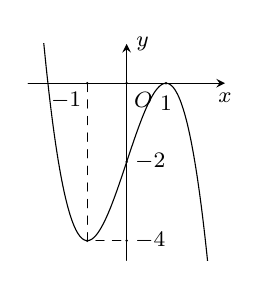
\begin{tikzpicture}[scale=.5, font=\footnotesize, line join=round, line cap=round, >=stealth]
    \draw[->] (-2.5,0)--(2.5,0) node[below] {$x$};
			\draw[->] (0,-4.5)--(0,1) node[right] {$y$};
			\draw[dashed] (-1,0)|-(0,-4);
			\clip (-2.5,-4.5) rectangle (2.5,1);
			\draw[smooth,samples=100,domain=-2.5:2.5] plot(\x,{-(\x)^3+3*\x-2});
			\foreach \x/\y/\ang/\dist/\lbl in {0/0/-45/0.3/O, -1/0/-140/0.35/-1, 1/0/-90/0.25/1, 0/-4/0/0.3/-4, 0/-2/0/0.3/-2, 0/2/180/0.2/2} \fill (\x,\y) circle (1pt) node[shift={(\ang:\dist)}] {$\lbl$};
			\fill (-1,-4) circle (1pt);
    \end{tikzpicture}
		}
	\loigiai{
		Ta có $y' = -3x^2+3$ và $y'' = -6x$.\\
		Khi đó, $y'' = 0 \Leftrightarrow -6x = 0 \Leftrightarrow x = 0 \Rightarrow y = -2$.\\
		Vậy tâm đối xứng của đồ thị hàm số là điểm $J(0;-2)$.
	}
\end{ex}

\begin{ex}%[1H4N6-2]
	\immini{Cho hình hộp $ABCD.A'B'C'D'$. Xét phép chiếu song song theo phương $A'A$ lên mặt phẳng $(ABCD)$. Ảnh của đoạn thẳng $A'C'$ qua phép chiếu song song đó là
		\choice
			{đoạn thẳng $A'C$}
			{đoạn thẳng $AB$}
			{đoạn thẳng $BD$}
			{\True đoạn thẳng $AC$}}{
		\begin{tikzpicture}[scale=1, font=\footnotesize, line join=round,
    line cap=round, >=stealth]
			\def \goc{225}  \def \gocx{80} \def \a{1.35} \def \b{3.25} \def \h{2}
			\path 
				(0,0) coordinate (A)
				(\b,0) coordinate (B)
				(\goc:\a) coordinate (D)
				($(D)+(B)-(A)$) coordinate (C)
				(\gocx:\h) coordinate (A')
				($(\gocx:\h)+(B)$) coordinate (B')
				($(\gocx:\h)+(D)$) coordinate (D')
				($(\gocx:\h)+(C)$) coordinate (C'); 
			\draw[dashed] (D)--(A)--(B) (A)--(A');
			\draw (D)--(C)--(B)--(B')--(A')--(D')--(C')--(C) (D)--(D') (B')--(C');
			\foreach \x/\g in {A/150, B/0, C/-60, D/-135, A'/120, B'/45, C'/-15, D'/180 }{\fill (\x) circle (1pt) node[shift={(\g:7pt)}]{$\x$};}
    \end{tikzpicture}
		}
	\loigiai{
		\begin{center}
			\begin{tikzpicture}[scale=0.8, font=\footnotesize, line join=round,
    line cap=round, >=stealth]
				\def \goc{225}  \def \gocx{80} \def \a{1.35} \def \b{3.25} \def \h{2}
				\path 
					(0,0) coordinate (A)
					(\b,0) coordinate (B)
					(\goc:\a) coordinate (D)
					($(D)+(B)-(A)$) coordinate (C)
					(\gocx:\h) coordinate (A')
					($(\gocx:\h)+(B)$) coordinate (B')
					($(\gocx:\h)+(D)$) coordinate (D')
					($(\gocx:\h)+(C)$) coordinate (C'); 
				\draw[dashed] (D)--(A)--(B) (C)--(A)--(A') ;
				\draw (D)--(C)--(B)--(B')--(A')--(D')--(C')--(C) (D)--(D') (B')--(C')--(A');
				\foreach \x/\g in {A/150, B/0, C/-60, D/-135, A'/120, B'/45, C'/-15, D'/180 }{\fill (\x) circle (1pt) node[shift={(\g:7pt)}]{$\x$};}
    \end{tikzpicture}
		\end{center}
		Qua phép chiếu song song theo phương $A'A$ lên mặt phẳng $(ABCD)$, ta có
		\begin{itemize}
			\item Ảnh của điểm $A'$ là điểm $A$;
			\item Ảnh của điểm $C'$ là điểm $C$ (vì $C'C \parallel A'A$).
		\end{itemize}
		Do đó, ảnh của đoạn thẳng $A'C'$ là đoạn thẳng $AC$.
	}
\end{ex}

\begin{ex}%[1D2H1-4]
	Trong các dãy số có số hạng tổng quát sau đây, dãy số nào là dãy số tăng?
	\choice
		{$\dfrac{1}{3^n}$}
		{\True $n+1$}
		{$1+\dfrac{1}{n}$}
		{$6-2n$}
	\loigiai{
		Xét dãy số $u_n = n+1$, ta có $u_{n+1} - u_n = (n+1+1) - (n+1) = 1 > 0$, $\forall n \in \mathbb{N}^*$.\\
		Vậy $u_n = n+1$ là dãy số tăng.
	}
\end{ex}

\begin{ex}%[1D6H4-3]
	Tập nghiệm của bất phương trình $\log_2(x-1)>3$ là
	\choice
		{$(1;+\infty)$}
		{$(1;9)$}
		{\True $(9;+\infty)$}
		{$(-\infty;9)$}
	\loigiai{
		Điều kiện xác định $x-1 > 0 \Leftrightarrow x > 1$.\\
		Ta có $\log_2(x-1)>3 \Leftrightarrow x-1 > 2^3 \Leftrightarrow x-1 > 8 \Leftrightarrow x > 9$.\\
		Kết hợp với điều kiện xác định, ta được $x > 9$.\\
		Vậy tập nghiệm của bất phương trình là $(9;+\infty)$.
	}
\end{ex}

\begin{ex}%[2H2H1-3]
	\immini{Cho hình lập phương $ABCD.A'B'C'D'$ có cạnh bằng $1$. Tích vô hướng của hai vectơ $\overrightarrow{CC'}$ và $\overrightarrow{A'A}$ bằng
		\choice[2]
			{$0$}
			{\True $-1$}
			{$2$}
			{$1$}}{
		\begin{tikzpicture}[scale=0.7, font=\footnotesize, line join=round,
    line cap=round, >=stealth]
			\def \goc{225}  \def \gocx{90} \def \a{1.25} \def \b{2.5} \def \h{2.25}
			\path 
				(0,0) coordinate (A)
				(\b,0) coordinate (B)
				(\goc:\a) coordinate (D)
				($(D)+(B)-(A)$) coordinate (C)
				(\gocx:\h) coordinate (A')
				($(\gocx:\h)+(B)$) coordinate (B')
				($(\gocx:\h)+(D)$) coordinate (D')
				($(\gocx:\h)+(C)$) coordinate (C'); 
			\draw[dashed] (D)--(A)--(B) (A)--(A');
			\draw (D)--(C)--(B)--(B')--(A')--(D')--(C')--(C) (D)--(D') (B')--(C');
			\foreach \x/\g in {A/150, B/0, C/-60, D/-135, A'/120, B'/45, C'/-15, D'/180 }{\fill (\x) circle (1pt) node[shift={(\g:7pt)}]{$\x$};}
    \end{tikzpicture}
		}
	\loigiai{
		Do $ABCD.A'B'C'D'$ là hình lập phương nên $\overrightarrow{A'A} = \overrightarrow{C'C} = -\overrightarrow{CC'}$.\\
		Khi đó $\overrightarrow{CC'} \cdot \overrightarrow{A'A} = \overrightarrow{CC'} \cdot \left(-\overrightarrow{CC'}\right) = -\left|\overrightarrow{CC'}\right|^2 = -1^2 = -1$.
	}
\end{ex}

\begin{ex}%[2H5N1-1]
	Trong không gian với hệ tọa độ $Oxyz$, phương trình nào sau đây là phương trình tổng quát của một mặt phẳng?
	\choice
		{$\dfrac{x-2}{2}=\dfrac{y-1}{2}=\dfrac{z}{1}$}
		{\True $x-1=0$}
		{$x^2+y^2+z^2-4=0$}
		{$\dfrac{2}{x}+\dfrac{1}{y}-\dfrac{3}{z}=0$}
	\loigiai{
		Phương trình tổng quát của mặt phẳng có dạng $Ax+By+Cz+D=0$ với $A^2+B^2+C^2>0$.\\
		Do đó, phương trình $x-1=0$ là phương trình của một mặt phẳng với $A=1$, $B=C=0$, $D=-1$.
	}
\end{ex}

\begin{ex}%[2H2H2-1]
	Trong không gian với hệ tọa độ $Oxyz$, cho $\vec{a}=-3\vec{i}+5\vec{j}+\vec{k}$. Độ dài của vectơ $\vec{a}$ bằng
	\choice
		{$\sqrt{17}$}
		{$35$}
		{$17$}
		{\True $\sqrt{35}$}
	\loigiai{
		Ta có $\vec{a}=-3\vec{i}+5\vec{j}+\vec{k} \Rightarrow \vec{a}=(-3;5;1)$.\\
		Độ dài của vectơ $\vec{a}$ là $\left|\vec{a}\right| = \sqrt{(-3)^2+5^2+1^2} = \sqrt{9+25+1} = \sqrt{35}$.
	}
\end{ex}
\Closesolutionfile{ans}
\cauds
\setcounter{ex}{0}
\Opensolutionfile{ans}[ans/ansDS-NgheAn-L1]
%%%%%%%%%%%%%%%%%%%%%%%%%%%%%%%%%%%%%%%%%%%%%%%%%%%%%%%%%
\begin{ex}%[2D1V3-6]
	Một hợp tác xã (viết tắt là HTX) nông nghiệp tại Nghệ An đầu tư dự án trồng dưa lưới nhà màng VietGAP. Xét trong một vụ canh tác, với diện tích $x$ (nghìn m$^2$, $x \geq 1$), tổng chi phí là $C(x)=x^2+30x+100$ (triệu đồng). Tổng doanh thu dự kiến là $R(x)=x^2+100x$ (triệu đồng).
	\choiceTF
		{\True Hàm số lợi nhuận của HTX sau một vụ canh tác là $L(x)=70x-100$ (triệu đồng)}
		{\True Nếu HTX muốn đạt mức lợi nhuận là $250$ triệu đồng cho một vụ thì diện tích canh tác cần thiết là $5$ nghìn m$^2$}
		{Chi phí trung bình trên mỗi đơn vị diện tích được định nghĩa là $P(x)=\dfrac{C(x)}{x}$. Khi diện tích canh tác tăng từ $1$ nghìn m$^2$ đến $11$ nghìn m$^2$ thì chi phí trung bình luôn giảm}
		{Để đồng vốn đầu tư đạt hiệu quả cao nhất (tỉ lệ lợi nhuận trên tổng chi phí $Q(x)=\dfrac{L(x)}{C(x)}$ đạt giá trị lớn nhất), HTX cần tính toán để chi phí trung bình trên mỗi đơn vị diện tích $P(x)$ đạt mức thấp nhất}
	\loigiai{
		\begin{itemchoice}
			\itemch Hàm số lợi nhuận của HTX sau một vụ canh tác là
			\allowdisplaybreaks
			\begin{align*}
				L(x)&=R(x)-C(x)\\
				&=\left(x^2+100x\right)-\left(x^2+30x+100\right)\\
				&=70x-100.
			\end{align*}
			Vậy lợi nhuận của HTX sau một vụ canh tác là $L(x)=70x-100$ (triệu đồng).
			\itemch Vì HTX muốn đạt mức lợi nhuận là $250$ triệu đồng cho một vụ nên ta có
			\allowdisplaybreaks
			\begin{eqnarray*}
				L(x)=250&\Leftrightarrow&70x-100=250\\
				&\Leftrightarrow&70x=350\\
				&\Leftrightarrow&x=5\ \left(\text{nghìn m$^2$}\right).
			\end{eqnarray*}
			Vậy HTX muốn đạt mức lợi nhuận là $250$ triệu đồng cho một vụ thì diện tích canh tác cần thiết là $5$ nghìn m$^2$.
			\itemch Ta có $P(x)=\dfrac{C(x)}{x}=\dfrac{x^2+30x+100}{x}$.\\
			Xét 
			\allowdisplaybreaks
			\begin{align*}
				P'(x)&=\left(\dfrac{x^2+30x+100}{x}\right)'\\
				&=\dfrac{\left(x^2+30x+100\right)'\cdot x-(x)'\cdot\left(x^2+30x+100\right)}{x^2}\\
				&=\dfrac{(2x+30)\cdot x-x^2-30x-100}{x^2}\\
				&=\dfrac{2x^2+30x-x^2-30x-100}{x^2}\\
				&=\dfrac{x^2-100}{x^2}.
			\end{align*}
			Suy ra $P'(x)=0\Leftrightarrow\dfrac{x^2-100}{x^2}=0\Leftrightarrow\hoac{&x=10\text{ (nhận)}\\&x=-10\text{ (loại)}.}$\\
			Bảng biến thiên
			\begin{center}
				
\begin{tikzpicture}
    \tkzTabInit[nocadre=true, lgt=1.3, espcl=4, deltacl=0.5]
					{$x$/0.7,$P'(x)$/0.7,$P(x)$/2}
					{$1$, $10$,$+\infty$}
					\tkzTabLine{,-,0,+,}
					\tkzTabVar{+/$131$,-/$50$,+/$+\infty$}
    \end{tikzpicture}
			\end{center}
			Do đó, diện tích canh tác tăng từ $1$ nghìn m$^2$ đến $10$ nghìn m$^2$ thì chi phí trung bình luôn giảm.
			\itemch Ta có $Q(x)=\dfrac{L(x)}{C(x)}=\dfrac{70x-100}{x^2+30x+100}$.\\
			Xét 
			\allowdisplaybreaks
			\begin{align*}
				Q'(x)&=\left(\dfrac{70x-100}{x^2+30x+100}\right)'\\
				&=\dfrac{(70x-100)'\cdot\left(x^2+30x+100\right)-\left(x^2+30x+100\right)'\cdot(70x-100)}{\left(x^2+30x+100\right)^2}\\
				&=\dfrac{70\cdot\left(x^2+30x+100\right)-(2x+30)\cdot(70x-100)}{\left(x^2+30x+100\right)^2}\\
				&=\dfrac{70x^2+2\,100x+7\,000-140x^2+200x-2\,100x+3\,000}{\left(x^2+30x+100\right)^2}\\
				&=\dfrac{-70x^2+200x+10\,000}{\left(x^2+30x+100\right)^2}.
			\end{align*}
			Suy ra $Q'(x)=0\Leftrightarrow\dfrac{-70x^2+200x+10\,000}{\left(x^2+30x+100\right)^2}=0\Leftrightarrow\hoac{&x=x_0=\dfrac{10+10\sqrt{71}}{7}\text{ (nhận)}\\&x=\dfrac{10-10\sqrt{71}}{7}\text{ (loại)}.}$\\
			Bảng biến thiên
			\begin{center}
				
\begin{tikzpicture}
    \tkzTabInit[nocadre=true, lgt=1.3, espcl=4, deltacl=0.6]
					{$x$/0.7,$Q'(x)$/0.7,$Q(x)$/2}
					{$1$, $x_0$,$+\infty$}
					\tkzTabLine{,+,0,-,}
					\tkzTabVar{-/$Q(1)$,+/$Q\left(x_0\right)$,-/$0$}
    \end{tikzpicture}
			\end{center}
			Suy ra hàm số $Q(x)$ đạt giá trị lớn nhất tại $x=x_0=\dfrac{10+10\sqrt{71}}{7}$ và hàm số $P(x)$ đạt giá trị nhỏ nhất tại $x=10$.\\
			Vậy hàm số $Q(x)$ đạt giá trị lớn nhất tại $x=x_0=\dfrac{10+10\sqrt{71}}{7}$ không trùng với hàm số $P(x)$ đạt giá trị nhỏ nhất tại $x=10$.
		\end{itemchoice}
	}
\end{ex}

\begin{ex}%[2D1H5-1]
	\immini{Cho hàm số $y=f(x)=-x-\dfrac{1}{x-1}$ có đồ thị là đường cong $(C)$.
		\choiceTF
			{\True Đường thẳng $x=1$ là tiệm cận đứng của đường cong $(C)$}
			{$f'(x)=\dfrac{-x^2+2x}{x-1}$, $\forall x\neq 1$}
			{Điểm cực đại của đồ thị hàm số là $N(2; 3)$}
			{Đường cong $(C)$ có dạng như hình vẽ}
		}
			{\begin{tikzpicture}[scale=0.8, font=\footnotesize,line join=round, line cap=round, >=stealth, x=0.6cm, y=0.6cm]
    \def\xt{-3} \def\xp{5} \def\yt{5} \def\yd{-3}
				\tikzset{declare function = {f(\x)= \x+1/(\x-1);}}
				\draw[->] (\xt,0)--(\xp,0) node [below]{$x$};
				\draw[->] (0,\yd)--(0,\yt) node [left]{$y$};
				\node at (0,0) [below right]{$O$};
				\fill (0,0) circle(1pt);
				\begin{scope}
					\clip (\xt,\yd) rectangle (\xp,\yt);
					\draw[smooth,samples=200,domain=\xt:0.9] plot(\x,{f(\x});
					\draw[smooth,samples=200,domain=1.1:\xp] plot(\x,{f(\x});
					\draw (1,\yd)--(1,\yt);
					\draw plot[domain=\xt:\xp] (\x,{\x}); 
				\end{scope}
				\foreach \diem/\pos/\name in {(1,0)/-60/1, (2,0)/-90/2, (3,0)/-90/3, (4,0)/-90/4, (0,1)/180/1, (0,2)/180/2, (0,3)/180/3, (0,4)/180/4} \fill \diem node[shift={(\pos:2.5mm)}]{$\name$} circle(1pt);
				\foreach \diem/\pos/\name in {(-2,0)/-110/-2, (-1,0)/-110/-1, (0,-2)/180/-2, (0,-1)/150/-1} \fill \diem node[shift={(\pos:3mm)}]{$\name$} circle(1pt);
    \end{tikzpicture}}
	\loigiai{
		\begin{itemchoice}
			\itemch Tập xác định $\mathscr{D}=\mathbb{R}\setminus\{1\}$.\\
			Ta có
			\begin{itemize}
				\item $\displaystyle\lim\limits_{x\to1^{+}}\left(-x-\dfrac{1}{x-1}\right)=\displaystyle\lim\limits_{x\to1^{+}}\left(\dfrac{-x^2+x-1}{x-1}\right)=-\infty$.
				\item $\displaystyle\lim\limits_{x\to1^{-}}\left(-x-\dfrac{1}{x-1}\right)=\displaystyle\lim\limits_{x\to1^{-}}\left(\dfrac{-x^2+x-1}{x-1}\right)=+\infty$.
			\end{itemize}
			Suy ra đồ thị hàm số $y=-x-\dfrac{1}{x-1}$ có tiệm cận đứng là đường thẳng $x=1$.
			\itemch Với $x\ne 1$, ta có 
			\allowdisplaybreaks
			\begin{align*}
				y'&=\left(-x-\dfrac{1}{x-1}\right)'\\
				&=-1+\dfrac{1}{(x-1)^2}\\
				&=\dfrac{-(x-1)^2+1}{(x-1)^2}\\
				&=\dfrac{-x^2+2x}{(x-1)^2}.
			\end{align*}
			Vậy $y'=f'(x)=\dfrac{-x^2+2x}{(x-1)^2}$, $\forall x\ne1$.
			\itemch Ta có $y'=0\Leftrightarrow\dfrac{-x^2+2x}{(x-1)^2}=0\Leftrightarrow\hoac{&x=0\\&x=2.}$\\
			Bảng biến thiên
			\begin{center}
				
\begin{tikzpicture}
    \tkzTabInit[nocadre=true, lgt=1.0, espcl=2.5, deltacl=0.5]
					{$x$/0.7,$y'$/0.7,$y$/2}
					{$-\infty$,$0$,$1$,$2$,$+\infty$}
					\tkzTabLine{,-,0,+,d,+,0,-,}
					\tkzTabVar{+/$+\infty$,-/$1$,+D-/$+\infty$/$-\infty$,+/$-3$,-/$+\infty$}
    \end{tikzpicture}
			\end{center}
			Dựa vào bảng biến thiên, ta thấy hàm số $y=f(x)$ đạt cực đại tại $x=2$ và giá trị cực đại là $y=-3$.\\
			Vậy điểm cực đại của đồ thị hàm số là $N(2;-3)$.
			\itemch Đồ thị của hàm số $y=f(x)=-x-\dfrac{1}{x-1}$ có
			\begin{itemize}
				\item Tiệm cận đứng là đường thẳng $x=1$.
				\item Tiệm cận xiên là đường thẳng $y=-x$.
				\item Hai điểm cực trị là điểm cực tiểu $(0;1)$ và điểm cực đại $(2;-3)$.
			\end{itemize}
			Vậy đường cong $(C)$ có dạng như hình vẽ sau:
			\begin{center}
				\begin{tikzpicture}[scale=1, font=\footnotesize,line join=round, line cap=round, >=stealth, x=0.6cm, y=0.6cm]
    \def\xt{-3} \def\xp{5} \def\yt{5} \def\yd{-6}
					\tikzset{declare function = {f(\x)= -\x-1/(\x-1);}}
					\draw[->] (\xt,0)--(\xp,0) node [below]{$x$};
					\draw[->] (0,\yd)--(0,\yt) node [left]{$y$};
					\node at (0,0) [below left]{$O$};
					\fill (0,0) circle(1pt);
					\begin{scope}
						\clip (\xt,\yd) rectangle (\xp,\yt);
						\draw[smooth,samples=200,domain=\xt:0.9] plot(\x,{f(\x});
						\draw[smooth,samples=200,domain=1.1:\xp] plot(\x,{f(\x});
						\draw (1,\yd)--(1,\yt);
						\draw plot[domain=\xt:\xp] (\x,{-\x}); 
					\end{scope}
					\foreach \diem/\pos/\name in {(-2,0)/-110/-2, (-1,0)/-110/-1, (2,0)/-90/2, (3,0)/-90/3, (4,0)/-90/4, (0,2)/-160/2, (0,3)/-160/3, (0,4)/-160/4}
					\fill \diem node[shift={(\pos:2.5mm)}]{$\name$} circle(1pt);
					\foreach \diem/\pos/\name in {(1,0)/-60/1, (0,1)/-150/1, (0,-1)/180/-1, (0,-2)/180/-2, (0,-3)/180/-3, (0,-4)/180/-4, (0,-5)/180/-5}
					\fill \diem node[shift={(\pos:3mm)}]{$\name$} circle(1pt);
    \end{tikzpicture}
			\end{center}
		\end{itemchoice}
	}
\end{ex}

\begin{ex}%[2H5V2-8]
	\immini{
	Trong một mô hình nông nghiệp công nghệ cao, một tấm pin năng lượng mặt trời phẳng được lắp đặt nghiêng sao cho bề mặt của nó nằm trên mặt phẳng $(P)\colon 2x+2y+z-6=0$ (xét trong hệ không gian tọa độ $Oxyz$ với đơn vị đo là mét, mặt phẳng $(Oxy)$ được xem là mặt đất phẳng). Người ta lắp đặt một robot cố định ở trên cao để kiểm tra bụi bẩn. Robot có mắt phát tia laser tại điểm $S(1;1;6)$. Robot thực hiện quét tia laser trên bề mặt tấm pin. Tại một thời điểm tia laser được chiếu theo đường thẳng $\Delta$ có vectơ chỉ phương $\vec{u}=(1;-2;-2)$ và chạm vào bề mặt tấm pin tại điểm $M$.
	}{
		\begin{tikzpicture}[scale=0.7, font=\footnotesize, line join=round, line cap=round, >=stealth]
			\definecolor{deepskyblue}{rgb}{0.0, 0.75, 1.0}
			\fill[bottom color=gray!10,top color=deepskyblue!90, middle color=white] (-3,-4) rectangle (6,3.5);
			\def \gx{170} \def \gy{15} 
			% Cột robot
			\draw[fill=gray!15] (-1,-2)--(-1,3)--++(-\gx:0.1)--++(-90:5)--cycle;
			\draw[fill=gray!30] (-1,-2)--++(-\gy:0.15)--++(90:5	)--(-1,3)--cycle;
			\draw[fill=gray!30] (-0.97,2.4)--++(-\gy:0.15)--++(90:0.4)--++(180-\gy:0.15)--cycle;
			\draw[fill=gray!50!brown!20] (-0.97,2.6)--++(55:0.22)coordinate(C1)--++(-50:0.4)coordinate(C2)--++(-125:0.22)coordinate(C3)--cycle
			(C1)--++(-\gy:0.15)--++(-50:0.4)coordinate(C4)--(C2)--cycle
			(C4)--(C2)--(C3)--($(C3)-(C2)+(C4)$)--cycle
			;
			\coordinate (LensBase) at ($(C2)!0.5!($(C3)-(C2)+(C4)$)$);
			\begin{scope}[shift={(LensBase)}, rotate=-50]
				\fill[black!80] (0, 0.09) -- (0.15, 0.09) -- (0.15, -0.09) -- (0, -0.09) -- cycle;
				\fill[black!80] (0, 0) ellipse [x radius=0.035, y radius=0.09]; 
				\draw[] (0, 0.09) -- (0.15, 0.09) (0, -0.09) -- (0.15, -0.09);
				\draw[fill=black!95] (0.15, 0) ellipse [x radius=0.035, y radius=0.09];
				\draw[fill=blue!50!cyan] (0.15, 0) ellipse [x radius=0.025, y radius=0.075];
				\fill[white, opacity=0.7] (0.15, 0.015) ellipse [x radius=0.01, y radius=0.02];
			\end{scope}
			% ================= Tấm pin
			\def \gp{45} 
			\path (-2,-2) coordinate (P1)
			++(\gp:3) coordinate (P2)
			++(\gx-177:5) coordinate (P3)
			++(\gp-180:3.3) coordinate (P4)
			;
			\def\hstand{0.5} % Chiều cao từ đất lên mép dưới
			% Giá đỡ
			\path
			coordinate (A_FL) at ($(P1)!0.08!(P4)$)
			coordinate (A_FR) at ($(P4)!0.08!(P1)$)
			coordinate (A_RL) at ($(P1)!0.75!(P2)$)
			coordinate (A_RR) at ($(P4)!0.55!(P3)$)
			coordinate (B1)   at ($(A_FL)+(0,-\hstand)$)
			coordinate (B4)   at ($(A_FR)+(0,-\hstand)$)
			coordinate (B2)   at ($(B1)+(25:2)$)
			coordinate (B3)   at ($(B4)+(25:2)$);     
			\def\tw{0.15} % Độ dày ống thép
			% Thanh đáy bên trái
			\draw[fill=gray!20] (B1) -- (B2) -- ($(B2)+(-10:\tw)$) -- ($(B1)+(-10:\tw)$) -- cycle;
			\draw[fill=gray!40] ($(B1)+(-10:\tw)$) -- ($(B2)+(-10:\tw)$) -- ($(B2)+(-10:\tw)+(0,-\tw)$) -- ($(B1)+(-10:\tw)+(0,-\tw)$) -- cycle;
			% Thanh đáy phía sau
			\draw[fill=gray!20] (B2) -- (B3) -- ($(B3)+(25:\tw)$) -- ($(B2)+(25:\tw)$) -- cycle;
			\draw[fill=gray!50] (B2) -- (B3) -- ($(B3)+(0,-\tw)$) -- ($(B2)+(0,-\tw)$) -- cycle;
			% Chân chống nghiêng bên phải 
			\draw[fill=gray!30] (B3) -- (A_RR) -- ($(A_RR)+(-\tw,0)$) -- ($(B3)+(-\tw,0)$) -- cycle;
			\draw[fill=gray!50] (B3) -- (A_RR) -- ($(A_RR)+(25:\tw)$) -- ($(B3)+(25:\tw)$) -- cycle;
			\draw[fill=gray!30] (B3) --($(B3)+(0,-\tw)$)--($(B3)+(0,-\tw)+(25:\tw)$)--($(B3)+(25:\tw)$)--cycle;
			\def\th{0.12} % Độ dày khung
			% Thanh đáy bên phải
			\draw[fill=gray!20] (B4) -- (B3) -- ($(B3)+(-\tw,0)$) -- ($(B4)+(-\tw,0)$) -- cycle;
			\draw[fill=gray!50] (B4) -- (B3) -- ($(B3)+(0,-\tw)$) -- ($(B4)+(0,-\tw)$) -- cycle;
			% Thanh đáy phía trước
			\draw[fill=gray!20] (B1) -- (B4) -- ($(B4)+(25:\tw)$) -- ($(B1)+(25:\tw)$) -- cycle;
			\draw[fill=gray!50] (B1) -- (B4) -- ($(B4)+(0,-\tw)$) -- ($(B1)+(0,-\tw)$) -- cycle;
			% Chân đứng phía trước bên phải 
			\coordinate (Leg1_Top) at ($(A_FR)+(0,-\th)$);
			\draw[fill=gray!30] (B4) -- (Leg1_Top) -- ($(Leg1_Top)+(\gx:\tw)$) -- ($(B4)+(\gx:\tw)$) -- cycle;
			\draw[fill=gray!50] (B4) -- (Leg1_Top) -- ($(Leg1_Top)+(25:\tw)$) -- ($(B4)+(25:\tw)$) -- cycle;
			% Chân đứng phía trước bên trái
			\coordinate (Leg2_Top) at ($(A_FL)+(0,-\th)$);
			\draw[fill=gray!30] (B1) -- (Leg2_Top) -- ($(Leg2_Top)+(\gx-180:\tw)$) -- ($(B1)+(\gx-180:\tw)$) -- cycle;
			\draw[fill=gray!50] ($(B1)+(\gx-180:\tw)$) -- ($(Leg2_Top)+(\gx-180:\tw)$) -- ($(Leg2_Top)+(25:\tw)+(\gx-180:\tw)$) -- ($(B1)+(25:\tw)+(\gx-180:\tw)$) -- cycle;
			% Mặt trên tấm pin
			\draw[fill=gray!50] (P3) -- (P4) -- ($(P4)+(0,-\th)$) -- ($(P3)+(0,-\th)$) -- cycle;
			\draw[fill=gray!30] (P1) -- (P4) -- ($(P4)+(0,-\th)$) -- ($(P1)+(0,-\th)$) -- cycle;
			\draw[fill=gray!20] (P1) -- (P2) -- (P3) -- (P4) -- cycle;
			\coordinate (I1) at ($(P1) + (\gx-180:0.1) + (\gp:0.1)$);
			\coordinate (I2) at ($(P2) + (\gx-180:0.1) - (\gp:0.1)$);
			\coordinate (I3) at ($(P3) - (\gx-180:0.1) - (\gp:0.1)$);
			\coordinate (I4) at ($(P4) - (\gx-180:0.1) + (\gp:0.1)$);
			\draw[fill=blue!50!cyan!50!black] (I1) -- (I2) -- (I3) -- (I4) -- cycle;
			\foreach \i in {1,...,5}{
				\draw[white!70, thin] ($(I1)!\i/6!(I2)$) -- ($(I4)!\i/6!(I3)$);
			}
			\foreach \j in {1,...,9}{
				\draw[white!70, thin] ($(I1)!\j/10!(I4)$) -- ($(I2)!\j/10!(I3)$);}
			\path (2.35,-1.5)coordinate (M);
			\fill[] (M) circle (1.5pt)node[shift=(-50:.25)]{\everymath{\color{yellow}}$M$};
			\draw[->,thick,red] ($(LensBase)!0.15cm!(M)$) --($(LensBase)!1cm!(M)$)node[shift=(60:0.3)]{$\vec{u}$};
			\draw[->,thick,red] ($(LensBase)!0.15cm!(M)$) --(M);
			\path ($(LensBase)!0.15cm!(M)$)node[above right]{$S$ (Robot)} 
			($(LensBase)!2.65cm!(M)$) node[right]{$\Delta$ (Tia laser)};
			\draw (4,-0.5)--(4,1)node[above]{$(P)$ (Mặt phẳng tấm pin)};
		\end{tikzpicture}
	}
	\choiceTF
		{\True Khoảng cách từ mắt phát tia laser $S$ đến mặt phẳng $(P)$ bằng $\dfrac{4}{3}$ mét}
		{Điểm $M$ có tọa độ là $(1;1;2)$}
		{\True Góc $\alpha$ hợp bởi tia laser $\Delta$ và mặt phẳng $(P)$ thỏa mãn hệ thức $\sin\alpha = \dfrac{4}{9}$}
		{Khi vệ sinh, nước được phun trúng điểm chạm của tia laser trên tấm pin sẽ tạo thành dòng nước chảy trên bề mặt pin xuống đất theo hướng dốc nhất, quỹ đạo chảy của dòng nước nằm trên một đường thẳng. Đường thẳng đó có một vectơ chỉ phương là $\vec{v}=(1;1;3)$}
	\loigiai{
		\begin{itemchoice}
			\itemch Ta có $\mathrm{d}\big(S,(P)\big) = \dfrac{|2\cdot1+2\cdot1+6-6|}{\sqrt{2^2+2^2+1^2}} = \dfrac{4}{3}$ (m).\\
			Vậy khoảng cách từ mắt phát tia laser $S$ đến mặt phẳng $(P)$ bằng $\dfrac{4}{3}$ mét.
			\itemch Phương trình đường thẳng (tia laser) $\Delta$ đi qua $S(1;1;6)$ nhận $\vec{u}=(1;-2;-2)$ làm một vectơ chỉ phương có dạng là $\heva{&x=1+t \\&y=1-2t \\&z=6-2t}$, $t\in\mathbb{R}$.\\
			Vì $M$ thuộc $\Delta$ nên có toạ độ $M(1+t;1-2t;6-2t)$.\\
			Mà $M$ thuộc mặt phẳng $(P)$ nên ta có
			\allowdisplaybreaks
			\begin{eqnarray*}
				&& 2(1+t)+2(1-2t)+(6-2t)-6=0\\
				&\Leftrightarrow& -4t+4=0\\
				&\Leftrightarrow& t=1.
			\end{eqnarray*}
			Suy ra $M(2;-1;4)$. 
			\itemch Đường thẳng chứa tia laser có một vectơ chỉ phương là $\vec{u}=(1;-2;-2)$. \\
			Mặt phẳng $(P)$ có một vectơ pháp tuyến là $\vec{n}=(2;2;1)$. \\
			Suy ra
			\[\sin\alpha = \dfrac{\left|\vec{u}\cdot\vec{n}\right|}{\left|\vec{u}\right|\cdot\left|\vec{n}\right|} = \dfrac{\big|1\cdot 2 + (-2)\cdot 2 + (-2)\cdot 1\big|}{\sqrt{1^2+(-2)^2+(-2)^2}\cdot\sqrt{2^2+2^2+1^2}} = \dfrac{4}{9}.\]
			Vậy với $\alpha$ là góc hợp bởi tia laser $\Delta$ và mặt phẳng $(P)$ thì $\sin\alpha=\dfrac{4}{9}$.
			\itemch 
			\begin{center}
				\begin{tikzpicture}[scale=1, font=\footnotesize, line join=round, line cap=round, >=stealth, declare function={gocX=0; gocY=60; gocZ=90;}]
    \path
						(0,0) coordinate (O)
						(gocX:5) coordinate (X)
						(gocY:3.5) coordinate (Y)
						(gocZ:4) coordinate (Z)
						(gocX:1)++(gocY:1.5) coordinate (d_start)
						(gocX:4.5)++(gocY:1) coordinate (d_end)
						(gocX:3)++(gocY:4)++(gocZ:5) coordinate (M)
						(gocX:3)++(gocY:2) coordinate (H)
						($(d_start)!0.55!(d_end)$) coordinate (P)
						($(d_start)!0.2!(d_end)$) coordinate (N);
					\draw[fill=gray!5, draw=gray!30] (0,0) -- (gocX:5) -- ++(gocY:3.5) -- (gocY:3.5) -- cycle;
					\path (d_start)++(gocZ:3.5)++(gocX:1) coordinate (P_top1)
						(d_end)++(gocZ:3.5)++(gocX:1) coordinate (P_top2)
						($(P_top2)!0.2!(P_top1)$) coordinate (Q)
						($(d_start)!.63!(Q)$) coordinate (M)
						;
					\draw[fill=blue!5, fill opacity=0.4] (d_start) -- (d_end) -- (P_top2) -- (P_top1) -- cycle;
					\node at (P_top2) [below left] {$(P)$};
					\draw ($(d_start)!-0.2!(d_end)$) -- ($(d_start)!1.2!(d_end)$) node[right] {$d$};
					\draw (M) -- (N) (M) -- (P);
					\draw[dashed] (M) -- (H) (H) -- (P) (H) -- (N);
					\draw[->] (O) -- (X) node[below] {$x$};
					\draw[->] (O) -- (Y) node[above right] {$y$};
					\draw[->] (O) -- (Z) node[right] {$z$};
					\draw pic[draw,angle radius=2mm] {right angle = M--P--N};
					\draw pic[draw,angle radius=2mm] {right angle = M--H--P};
					\foreach \p/\g in {M/above, H/below right, P/below right, N/below, O/left}
					\fill (\p) circle (1pt) node[\g] {$\p$};
    \end{tikzpicture}
			\end{center}
			Gọi $d = (P) \cap (Oxy)$, kẻ $MP \perp d$ tại $P$ ($P \in d$), $N$ là điểm bất kỳ thuộc $d$, $H$ là hình chiếu của $M$ lên mặt phẳng $(Oxy)$.\\
			Ta có $\sin \widehat{MNH} = \dfrac{MH}{MN} \le \dfrac{MH}{MP}=\sin \widehat{MPH}$ (do $MP \le MN$).\\ 
			Góc nghiêng càng lớn thì đường nước chảy càng dốc, lúc này góc nghiêng lớn nhất khi \break $\sin \widehat{MNH} = \dfrac{MH}{MP}$.\\
			Dấu \lq\lq$=$\rq\rq xảy ra khi và chỉ khỉ $N \equiv P$.\\
			Ta có $\heva{&\vec{u}_d\perp \vec{k}\\&\vec{u}_d\perp \vec{n}_{(P)}}\Rightarrow \vec{u}_d = \left[\vec{k}, \vec{n}\right]=(-2;2;0)$.\\
			Lại có $\heva{&\vec{v}\perp \vec{u}_d\\&\vec{v}\perp \vec{n}_{(P)}}$ nên
			$\vec{v} = \left[\vec{u}_d, \vec{n}\right]=(2;2;-8)=2(1;1;-4)$.\\
			Vậy đường thẳng dốc nhất có một vectơ chỉ phương là $\vec{v}=(1;1;-4)$.	
		\end{itemchoice}
	}
\end{ex}

\begin{ex}%[2D3V1-2]
	Để tuyển chọn thành viên cho Câu lạc bộ Toán - Tin, nhà trường tổ chức một bài thi đánh giá năng lực (thang điểm $100$) cho $100$ học sinh. Kết quả điểm thi được thống kê trong bảng số liệu ghép nhóm gồm $6$ nhóm như sau:
	\begin{center}
		\begin{tabular}{|l|c|c|c|c|c|c|}
			\hline
			Điểm số & $[40; 50)$ & $[50; 60)$ & $[60; 70)$ & $[70; 80)$ & $[80; 90)$ & $[90; 100]$ \\
			\hline
			Số học sinh & $10$ & $15$ & $25$ & $30$ & $15$ & $5$ \\ 
			\hline
		\end{tabular}
	\end{center}
	An và Bình là hai học sinh tham gia thi, đạt số điểm lần lượt là $82$ điểm và $69{,}5$ điểm. Ban chủ nhiệm Câu lạc bộ đưa ra quy định phân loại dựa trên các chỉ số thống kê của toàn bộ mẫu số liệu như sau:
	\begin{itemize}
		\item Xếp loại \lq\lq xuất sắc\rq\rq: Điểm số lớn hơn hoặc bằng tứ phân vị thứ ba.
		\item Xếp loại \lq\lq tiềm năng\rq\rq: Điểm số từ mức điểm trung vị đến dưới tứ phân vị thứ ba.
		\item Xếp loại \lq\lq chưa đạt\rq\rq: Điểm số dưới mức điểm trung vị.
	\end{itemize}
	Một điều hết sức thú vị là không có học sinh nào có điểm số bằng một trong ba giá trị tứ phân vị.
	\choiceTF
		{\True Khoảng biến thiên của mẫu số liệu ghép nhóm này là $60$}
		{Điểm trung vị của $100$ học sinh tham gia kỳ thi là $71$ điểm}
		{\True Mặc dù Bình xếp loại chưa đạt, nhưng điểm số của Bình vẫn cao hơn mức điểm trung bình}
		{\True Để đánh giá chất lượng đề thi, ban tổ chức chọn ngẫu nhiên $4$ học sinh tham gia kỳ thi để phỏng vấn. Xác suất để trong $4$ học sinh được chọn có đầy đủ đại diện của ba nhóm xếp loại và luôn có mặt An là  $\dfrac{275}{14\,259}$}
	\loigiai{
		\begin{itemchoice}
			\itemch Khoảng biến thiên của mẫu số liệu ghép nhóm là $R = 100 - 40 = 60$. 
			\itemch Cỡ mẫu $n=100$. \\
			Trung vị $M_\text{e}$ của mẫu số liệu gốc là $\dfrac{x_{50} + x_{51}}{2}$, mà $x_{50}$ thuộc nhóm $[60; 70)$ và $x_{51}$ thuộc nhóm $[70; 80)$. Do đó, trung vị của mẫu số liệu ghép nhóm là $M_\text{e} = 70$.
			\itemch Từ bảng thống kê, ta lập được bảng giá trị đại diện sau:
			\begin{center}
				\begin{tabular}{|l|c|c|c|c|c|c|}
					\hline
					Điểm số & $[40; 50)$ & $[50; 60)$ & $[60; 70)$ & $[70; 80)$ & $[80; 90)$ & $[90; 100]$ \\ \hline
					Giá trị đại diện & $45$ & $55$ & $65$ & $75$ & $85$ & $95$ \\ \hline
					Số học sinh & $10$ & $15$ & $25$ & $30$ & $15$ & $5$ \\ \hline
				\end{tabular}
			\end{center}
			Điểm trung bình của mẫu số liệu ghép nhóm trên là 
			\[\overline{x} = \dfrac{10\cdot 45 + 15\cdot 55 + 25\cdot 65 + 30\cdot 75 + 15\cdot 85 + 5\cdot 95}{100} = \dfrac{6\,900}{100} = 69.\]
			Bình được $69{,}5$ nên có điểm số cao hơn mức điểm trung bình.
			\itemch Tứ phân vị thứ ba $Q_3$ của mẫn số liệu gốc là $x_{75} + x_{76}$, mà $x_{75}$ và $x_{76}$ đều thuộc nhóm $[70; 80)$. Do đó, tứ phân vị thứ ba của mẫu số liệu ghép nhóm là
			\[Q_3 = 70 + \dfrac{75 - 50}{30} \cdot 10=\dfrac{235}{3}\approx78{,}3.\]
			An được $82$ điểm nên thuộc nhóm xếp loại \lq\lq xuất sắc\rq\rq.\\
			Có $100$ học sinh tham gia thi, không có học sinh nào có điểm số bằng một trong ba tứ phân vị nên ta có
			\begin{itemize}
				\item Số học sinh chưa đạt là $50$;
				\item Số học sinh tiềm năng là $25$;
				\item Số học sinh xuất sắc là $25$ (trong đó có An).
			\end{itemize}
			Chọn ngẫu nhiên $4$ học sinh từ $100$ học sinh là một tổ hợp chập $4$ của $100$. \\
			Do đó, số phần tử của không gian mẫu là $n(\Omega)=\mathrm{C}_{100}^4$.\\
			Gọi $A$ là biến cố: \lq\lq Có đầy đủ đại diện của ba nhóm xếp loại và luôn có mặt An\rq\rq.\\ 
			Các trường hợp chọn $3$ người còn lại (khi đã có An) có thể xảy ra là
			\begin{enumerate}[\it TH 1:]
				\item Chọn $4$ học sinh trong đó có An (xuất sắc), $1$ học sinh chưa đạt, $1$ học sinh tiềm năng và thêm $1$ học sinh xuất sắc (khác An) có số kết quả là $\mathrm{C}_{50}^1 \cdot \mathrm{C}_{25}^1 \cdot \mathrm{C}_{24}^1$.
				\item Chọn $4$ học sinh trong đó có An (xuất sắc), $2$ học sinh chưa đạt và $1$ học sinh tiềm năng có số kết quả là $\mathrm{C}_{50}^2 \cdot \mathrm{C}_{25}^1$.
				\item Chọn $4$ học sinh trong đó có An (xuất sắc), $1$ học sinh chưa đạt và $2$ học sinh tiềm năng có số kết quả là $\mathrm{C}_{50}^1 \cdot \mathrm{C}_{25}^2$.
			\end{enumerate}
			Tổng số cách chọn thuận lợi cho biến cố $A$ là $n(A) = \mathrm{C}_{50}^1 \cdot \mathrm{C}_{25}^1 \cdot \mathrm{C}_{24}^1 + \mathrm{C}_{50}^2 \cdot \mathrm{C}_{25}^1 + \mathrm{C}_{50}^1 \cdot \mathrm{C}_{25}^2$.\\
			Xác suất trong $4$ người được chọn có đầy đủ đại diện của ba nhóm xếp loại và luôn có mặt An là
			\[\mathrm{P}(A) = \dfrac{n(A)}{n(\Omega)}= \dfrac{\mathrm{C}_{50}^1 \cdot \mathrm{C}_{25}^1 \cdot \mathrm{C}_{24}^1 + \mathrm{C}_{50}^2 \cdot \mathrm{C}_{25}^1 + \mathrm{C}_{50}^1 \cdot \mathrm{C}_{25}^2}{\mathrm{C}_{100}^4} = \dfrac{275}{14\,259}.\]
		\end{itemchoice}
	}
\end{ex}
\Closesolutionfile{ans}
\caukq
\setcounter{ex}{0}
\Opensolutionfile{ans}[ans/ansTLN-NgheAn-L1]
%%%%%%%%%%%%%%%%%%%%%%%%%%%%%%%%%%%%%%%%%%%%%%%%%%%%%%%%%
\begin{ex}%[2D4V3-5]
	Một kiến trúc sư thiết kế một hồ bơi vô cực có mặt trên của bể bơi nằm trong mặt phẳng $Oxy$ (đơn vị trên trục là mét). Một cạnh của hồ bơi dài $12$\,m nằm trên trục $Ox$; hai cạnh bên lần lượt nằm trên trục $Oy$ và đường thẳng $x=12$; cạnh còn lại (mặt vô cực) là một phần đồ thị của hàm số $y=-\dfrac{1}{18}x^2+\dfrac{2}{3}x+4$. Đáy hồ bơi không phẳng mà độ sâu tại điểm $(a;b)$ được tính theo công thức $h(a)=\dfrac{1}{4}a+1$ (mét). Thể tích nước tối đa mà hồ bơi có thể chứa bằng bao nhiêu m$^3$?
	\begin{center}
		\begin{tikzpicture}[scale=0.6, font=\footnotesize, line join=round, line cap=round, >=stealth, x={(1cm,0cm)}, y={(0.4cm,0.4cm)}, z={(0cm,-0.8cm)}, declare function={f(\x)=-1/18*(\x)^2 + 2/3*\x + 4; h(\x)=1/4*\x + 1; a=7.5;}]
    \draw[fill=cyan!15] (0,0,0) -- (12,0,0) -- (12,0,{h(12)}) -- (0,0,{h(0)}) -- cycle;%VM011
			\draw[fill=cyan!25] (12,0,0) -- (12,{f(12)},0) -- (12,{f(12)},{h(12)}) -- (12,0,{h(12)}) -- cycle;
			\draw[fill=cyan!15] (0,0,0) -- plot[domain=0:12, samples=50] (\x, {f(\x)}, 0) -- (12,0,0) -- cycle;
			\draw[dashed,fill=cyan!25] (a,0,0) -- (a,{f(a)},0) -- (a,{f(a)},{h(a)}) -- (a,0,{h(a)}) -- cycle;
			\draw[] (a,0,{h(a)})--(a,0,0) -- (a,{f(a)},0);
			\draw[->] (0,0,0) -- (14.5,0,0) node[below] {$x$};
			\draw[->] (0,0,0) -- (0,7,0) node[above] {$y$};
			\node[shift=(180:2mm)] at (0,0,0) {$O$};
			\draw[] plot[domain=0:12, samples=50] (\x, {f(\x)}, 0);
			\path (12,0,0) node[below left=-2pt] {$12$} -- (12,{f(12)},0);
			\node[above, rotate=4] at (4.2, {f(6.5)-0.3}, 0) {$y=-\dfrac{1}{18}x^2+\dfrac{2}{3}x+4$};
			\node[left] at (a,0,0.5) {$a$};
			\node[above left] at (a,{f(a)/1.3},0.3) {$b$};
			\draw[<->] (a, {f(a)+1}, 0) -- (a, {f(a)+1}, {h(a)}) node[midway, right] {$h(a)$};%VM-MT-15
			\draw[dash pattern=on 2pt off 1.pt] (a, {f(a)}, 0) -- (a, {f(a)+0.8}, 0);
			\draw[dash pattern=on 2pt off 1.pt] (a, {f(a)}, {h(a)}) -- (a, {f(a)+0.8}, {h(a)});
			\draw[dashed] plot[domain=0:12, samples=50] (\x, {f(\x)}, {h(\x)})
				(0,{f(0)},0) -- (0,{f(0)},{h(0)})--(0,0,{h(0)})
				;
    \end{tikzpicture}
	\end{center}
	\par\shortans{160}
	\loigiai{
		Mặt trên của hồ bơi là một hình phẳng $\mathscr{D}$ nằm trong mặt phẳng tọa độ $Oxy$, được giới hạn bởi trục hoành $y=0$, trục tung $x=0$; đường thẳng $x=12$ và đồ thị hàm số $y=-\dfrac{1}{18}x^2+\dfrac{2}{3}x+4$.\\
		Độ sâu của hồ bơi tại điểm có hoành độ $x=a$ chỉ phụ thuộc vào $a$, do đó mặt cắt của hồ bơi khi cắt bởi mặt phẳng vuông góc với trục $Ox$ tại điểm có hoành độ $x \in [0;12]$ là một hình chữ nhật có kích thước hai cạnh là $y=-\dfrac{1}{18}x^2+\dfrac{2}{3}x+4$ và $h(x)=\dfrac{1}{4}x+1$.\\
		Diện tích của mặt cắt hình chữ nhật là
		\[S(x)=y \cdot h(x)=\left(-\dfrac{1}{18}x^2+\dfrac{2}{3}x+4 \right) \left(\dfrac{1}{4}x+1\right).\]
		Thể tích nước tối đa mà hồ bơi có thể chứa là
		\allowdisplaybreaks
		\begin{align*}
			V &= \displaystyle\int\limits_0^{12} S(x) \mathrm{\,d}x \\
			&= \displaystyle\int\limits_0^{12} \left(-\dfrac{1}{18}x^2+\dfrac{2}{3}x+4 \right) \left(\dfrac{1}{4}x+1\right) \mathrm{d}x \\
			&= 160.
		\end{align*}
		Vậy thể tích nước tối đa mà hồ bơi có thể chứa là $160$\,m$^3$.
	}
\end{ex}

\begin{ex}%[2H5C2-8]
	Một nhân viên cứu hộ đứng ở mặt đất, điều khiển một drone chở vật tư y tế, dự kiến bay thẳng từ đỉnh $A$ của tháp thứ nhất đến đỉnh $B$ của tháp thứ hai. Tuy nhiên, do gặp một khu vực nhiễu sóng an ninh nên drone phải bay thẳng từ $A$ đến một điểm $P$ trên mặt đất để hạ cánh. Nhân viên đó mang drone từ điểm $P$ dọc theo hướng Tây $40$\,m đến điểm $Q$ và sau đó drone bay thẳng từ điểm $Q$ lên đỉnh $B$ của tháp thứ hai (hình vẽ). Biết đỉnh $A$ cao $100$\,m và có hình chiếu lên mặt đất cách vị trí người đứng ban đầu $200$\,m về phía Đông và $100$\,m về phía Nam. Đỉnh $B$ cao $300$\,m và có hình chiếu lên mặt đất cách vị trí người đứng ban đầu $140$\,m về phía Tây và $200$\,m về phía Nam.
	\begin{center}
		\begin{tikzpicture}[scale=0.6, font=\footnotesize, line join=round, line cap=round, >=stealth]
    \def\dx{1.2} \def\dy{0.6} % Kích thước đáy khối dưới
			\def\tx{0.9} \def\ty{0.45} % Kích thước đáy khối trên
			\def\h{1.2}              % Chiều cao chóp
			% ============= THÁP VM015
			\newcommand{\tower}[7]{
			\def\x{#1} \def\y{#2} \def\lh{#3} \def\uh{#4}
			\def\by{\y+\lh} \def\py{\by+\uh}
			\pgfmathsetmacro{\H}{\lh + \uh + \h-0.85}
			\pgfmathsetmacro{\Hu}{\lh + \uh-0.5}
			\fill[black!20] (\x+\dx, \y+\dy)
				-- (\x, \y)
				-- (\x - 0.85*\lh, \y - 0.25*\lh)
				--++(150:0.1)
				-- (\x - 0.85*\Hu, \y - 0.25*\Hu+0.1)
				-- (\x - 0.85*\H, \y+\ty - 0.25*\H)
				-- (\x - 0.85*\Hu-\ty+0.1, \y - 0.25*\Hu+\tx-0.2)
				-- (\x - 0.85*\lh-\ty, \y - 0.25*\lh+\tx-0.2)
				--++(120:0.1)
				-- (\x, \y+2*\dy-0.2) -- cycle;
			\draw[fill=black!25] (\x-\dx, \y+\dy+\lh) -- (\x, \y+\lh) -- (\x+\dx, \y+\dy+\lh) -- (\x, \y+2*\dy+\lh) -- cycle;
			\draw[fill=black!40] (\x, \y) -- (\x-\dx, \y+\dy) -- (\x-\dx, \y+\dy+\lh) -- (\x, \y+\lh) -- cycle;
			\draw[fill=black!15] (\x, \y) -- (\x+\dx, \y+\dy) -- (\x+\dx, \y+\dy+\lh) -- (\x, \y+\lh) -- cycle;
			\foreach \i in {1,...,#5} {
			\pgfmathsetmacro{\cY}{\y + \lh*\i/(#5+1)}
			\draw[] (\x-\dx, \cY+\dy) -- (\x, \cY) -- (\x+\dx, \cY+\dy);
			}
			\begin{scope}[shift={(0,0.125)}]
				\draw[fill=black!25] (\x-\tx, \by+\ty+\uh) -- (\x, \by+\uh) -- (\x+\tx, \by+\ty+\uh) -- (\x, \by+2*\ty+\uh) -- cycle;
				\draw[fill=black!40] (\x, \by) -- (\x-\tx, \by+\ty) -- (\x-\tx, \by+\ty+\uh) -- (\x, \by+\uh) -- cycle;
				\draw[fill=black!15] (\x, \by) -- (\x+\tx, \by+\ty) -- (\x+\tx, \by+\ty+\uh) -- (\x, \by+\uh) -- cycle;
				\foreach \i in {1,...,#6} {
				\pgfmathsetmacro{\cY}{\by + \uh*\i/(#6+1)}
				\draw[] (\x-\tx, \cY+\ty) -- (\x, \cY) -- (\x+\tx, \cY+\ty);
				}
				\coordinate (#7) at (\x, \py+\h);
				\draw[fill=cyan!40!gray!60] (\x-\tx, \py+\ty) -- (\x, \py) -- (#7) -- cycle;
				\draw[fill=cyan!20!gray!30] (\x+\tx, \py+\ty) -- (\x, \py) -- (#7) -- cycle;
			\end{scope}
			}
			\tower{0}{0}{2.8}{1.8}{4}{2}{A}
			\tower{12.5}{1.5}{4.2}{2.8}{5}{3}{B}
			% =========== NGƯỜI VM015
			\begin{scope}[shift={(4, -2.5)}, scale=0.45]
				\begin{scope}[cm={1.2, 0, -1, -0.5, (0,0)}]
					\fill[black!20, rounded corners=0.5pt] (-0.25,0)--(-0.15,0)--(-0.05,1.2)--(-0.35,1.2)--cycle;
					\fill[black!20, rounded corners=0.5pt] (0.25,0)--(0.15,0)--(0.05,1.2)--(0.35,1.2)--cycle;   
					\fill[black!20, rounded corners=1pt] (-0.45,1.2)--(0.45,1.2)--(0.35,2.6)--(-0.35,2.6)--cycle; 
					\fill[black!20, rounded corners=1pt] (-0.35,2.5)--(-0.55,2.3)--(-0.5,1.3)--(-0.3,1.5)--cycle;
					\fill[black!20, rounded corners=1pt] (0.35,2.5)--(0.55,2.3)--(0.5,1.3)--(0.3,1.5)--cycle;    
					\fill[black!20] (0,3.0) ellipse (0.25 and 0.35); 
				\end{scope}
				\fill[black!75, rounded corners=0.5pt] (-0.25,0)--(-0.15,0)--(-0.05,1.2)--(-0.35,1.2)--cycle; 
				\fill[black!75, rounded corners=0.5pt] (0.25,0)--(0.15,0)--(0.05,1.2)--(0.35,1.2)--cycle;   
				\fill[black!85, rounded corners=1pt] (-0.45,1.2)--(0.45,1.2)--(0.35,2.6)--(-0.35,2.6)--cycle; 
				\fill[black!85, rounded corners=1pt] (-0.35,2.5)--(-0.55,2.3)--(-0.5,1.3)--(-0.3,1.5)--cycle; 
				\fill[black!85, rounded corners=1pt] (0.35,2.5)--(0.55,2.3)--(0.5,1.3)--(0.3,1.5)--cycle;   
				\fill[black!80] (0,3.0) ellipse (0.25 and 0.35); 
			\end{scope}
			%---
			\path (3.2, -0.3) coordinate (P) (4.8, -0.45) coordinate (Q);
			\foreach \x/\y in {A/P,P/Q,Q/B}{\draw[red,->] (\x) -- (\y);}
			\foreach \t/\g in {A/90,B/90,P/-90,Q/-90}{
			\fill (\t) circle (1.5pt) node[shift={(\g:8pt)}]{$\t$};}
			\foreach \d/\t in {(0.3,-0.5)/Tháp $1$, (12.75,.9)/Tháp $2$,(6, -2)/Người đứng}{\node[] at  \d {\t};}
    \end{tikzpicture}
	\end{center}
	Chọn hệ trục tọa độ $Oxyz$ có gốc tại vị trí người đứng ban đầu, mặt phẳng $(Oxy)$ là mặt đất, trục $Ox$ hướng Đông, trục $Oy$ hướng Nam và trục $Oz$ hướng thẳng đứng lên trên (đơn vị trên các trục là $100$\,m). Để hoàn thành nhiệm vụ, người đó chọn vị trí điểm $P(a;b;c)$ trên mặt đất sao cho tổng quãng đường bay là ngắn nhất. Giá trị của biểu thức $S=2a+4b+c$ bằng bao nhiêu?
	\par\shortans{7,5}
	\loigiai{
		Đổi các đơn vị khoảng cách theo hệ trục đã chọn (1 đơn vị $= 100$\,m).\\
		Khi đó $A(2;1;1)$ và $B(-1{,}4;2;3)$.\\
		Điểm $P$ nằm trên mặt đất $(Oxy)$ nên có cao độ $c=0$. Do đó, toạ độ điểm $P$ có dạng $(a;b;0)$.\\
		Điểm $Q$ có được bằng cách dịch chuyển $P$ theo hướng Tây $40$\,m tương ứng với $0{,}4$ đơn vị nên $Q(a-0{,}4;b;0)$.\\
		Tổng quãng đường bay của drone là $d = AP + QB$. Ta cần tìm $a$, $b$ để $d$ đạt giá trị nhỏ nhất.
		\begin{enumerate}[\bf Cách 1:]
			\item 
			Ta có $AP=\sqrt{(a-2)^2+(b-1)^2+(0-1)^2} = \sqrt{(2-a)^2+(1-b)^2+1}$ và 
			\allowdisplaybreaks
			\begin{align*}
				QB &= \sqrt{\big(-1{,}4-(a-0{,}4)\big)^2 + (2-b)^2 + (3-0)^2} \\
				&= \sqrt{(-1-a)^2+(2-b)^2+9} \\
				&= \sqrt{(a+1)^2+(b-2)^2+3^2}.
			\end{align*}
			Khi đó \[d =\sqrt{(2-a)^2+(1-b)^2+1^2} + \sqrt{(a+1)^2+(b-2)^2+3^2}.\]
			Xét hai vectơ $\vec{u}=(2-a;1-b;1)$ và $\vec{v}=(a+1;b-2;3)$.\\
			Ta có $\vec{u}+\vec{v}=(3;-1;4)$.\\
			Áp dụng bất đẳng thức, ta có độ dài vectơ $\left|\vec{u}\right|+ \left|\vec{v}\right| \ge \left|\vec{u} + \vec{v}\right|$, ta có
			\[d=\left|\vec{u}\right| + \left|\vec{v}\right| \ge \sqrt{3^2 + (-1)^2 + 4^2} = \sqrt{26}.\]			
			Dấu \lq\lq$=$\rq\rq \, xảy ra khi và chỉ khi $\vec{u}$ và $\vec{v}$ cùng hướng, tức là tồn tại $k\ge 0$ sao cho $\vec{u}=k\vec{v}$. Khi đó
			\[\heva{&2-a=k(a+1)\\&1-b=k(b-2)\\&1=3k} \Leftrightarrow \heva{&k=\dfrac{1}{3}\\&2-a=\dfrac{1}{3}(a+1)\\&1-b=\dfrac{1}{3}(b-2)} \Leftrightarrow \heva{&k=\dfrac{1}{3}\\&a=1{,}25\\&b=1{,}25.}\]
			Vậy $S=2a+4b+c=2\cdot 1{,}25+4\cdot 1{,}25+0 =7{,}5$.
			\item Ta có $AP=\sqrt{(a-2)^2+(b-1)^2+(0-1)^2}$ và 
			\allowdisplaybreaks
			\begin{align*}
				QB &= \sqrt{(-1{,}4-(a-0{,}4))^2 + (2-b)^2 + (3-0)^2} \\
				&=\sqrt{(-1-a)^2+(2-b)^2+(3-0)^2}.
			\end{align*}
			Khi đó
			\allowdisplaybreaks
			\begin{align*}
				d&=AP+QB\\
				&=\sqrt{(a-2)^2+(b-1)^2+(0-1)^2}+\sqrt{(-1-a)^2+(2-b)^2+(3-0)^2}\\
				&=AP+PK,
			\end{align*}
			trong đó $A(2;1;1)$; $P(a;b;0)$ và $K(-1;2;3)$.\\
			Nhận thấy $z_A>0$ và $z_K>0$ nên $A$ và $K$ nằm cùng phía so với mặt phẳng $(Oxy)$.\\
			Lấy đối xứng điểm $K$ qua mặt phẳng $(Oxy)$, ta được $K'(-1;2;-3)$.
			\begin{center}
				\begin{tikzpicture}[scale=0.6, font=\footnotesize, line join=round,
    line cap=round, >=stealth]
					\def \a{6}
					\def \h{2.5}
					\path
						(0,0) coordinate (O)
						(\a,0) coordinate (M)
						(\a+2,\h) coordinate (N)
						(2,\h) coordinate (Q)
						(2.5,4) coordinate (K)
						(2.5,-1.6) coordinate (K')
						(2.5,1.2) coordinate (H)
						(2.5,0) coordinate (H')
						(6,3) coordinate (A)
						($(H)+(4,0)$) coordinate (L)
						(intersection of H--L and A--K') coordinate (P)
						(intersection of O--M and A--K') coordinate (P'')
						;
					\draw (O)--(M)--(N)--(Q)--cycle (K)--(H) (H')--(K') (K)--(P)--(A) (P'')--(K');
					\draw[dashed,fill] (H) circle(1pt)-- (H') (P)--(P'');
					\foreach \x/\goc in {K/90,K'/-90,A/90,P/-45}
					\fill (\x) circle (1pt)
						($(\x)+(\goc:3mm)$)node{$\x$};
					\draw pic[draw,angle radius=2mm]{right angle=P--H--K};
					\draw pic[draw,angle radius=12mm]{angle=M--O--Q};
					\draw pic["$Oxy$",-stealth,angle radius=14mm]{angle=M--O--Q};
    \end{tikzpicture}
			\end{center}
			Do $(Oxy)$ là mặt phẳng trung trực của đoạn $KK'$ nên với $P \in (Oxy)$ thì $PK=PK'$.\\
			Suy ra $d=AP+PK' \ge AK'$.\\
			Dấu \lq\lq $=$\rq\rq \, xảy ra khi $P=AK' \cap (Oxy)$.\\
			Ta có $\overrightarrow{AK'}=(-3;1;-4)$.\\
			Đường thẳng $AK'$ đi qua $A(2;1;1)$ và nhận vectơ $\overrightarrow{AK'}=(-3;1;-4)$ là một vectơ chỉ phương nên $AK'$ có phương trình
			\[\heva{&x=2-3t\\&y=1+t\\&z=1-4t.}\]
			Giao điểm $P(x;y;z)$ của $AK'$ và $(Oxy)$ thỏa 
			\[z=0 \Leftrightarrow 1-4t=0 \Leftrightarrow t=0{,}25.\]
			Suy ra tổng quãng đường bay ngắn nhất thì $P(1{,}25;1{,}25;0)$.\\
			Do đó $a=1{,}25$; $b=1{,}25$ và $c=0$.\\
			Vậy  $S=2a+4b+c=2\cdot 1{,}25+4\cdot 1{,}25+0 =7{,}5$.
		\end{enumerate}
	}
\end{ex}

\begin{ex}%[0D2V2-3]
	Một doanh nghiệp phân bổ ngân sách quảng cáo trên Facebook và Google với tổng số tiền không vượt quá $80$ triệu đồng. Chi phí cho Facebook nằm trong khoảng từ $20$ đến $50$ triệu đồng. Chi phí cho Google tối thiểu là $15$ triệu đồng. Số tiền chi cho chạy quảng cáo trên Google không được vượt quá chi phí chi cho quảng cáo trên Facebook. Biết rằng số khách tiếp cận là $4$ nghìn khách cho mỗi triệu tiền chi quảng cáo trên Facebook và $6$ nghìn khách cho mỗi triệu quảng cáo trên Google. Hỏi số lượng khách tiếp cận lớn nhất bằng bao nhiêu nghìn?
	\par\shortans{400}
	\loigiai{
		Gọi $x$ (triệu đồng) là số tiền chi phí cho Facebook; $y$ (triệu đồng) là số tiền chi phí cho Google.\\
		Theo đề bài, ta có hệ điều kiện: $\heva{&x+y\le 80\\ &20\le x\le 50\\ &y\ge 15\\ &y\le x.}\quad (I)$\\
		Dễ thấy điểm $M(40;20)$ thuộc miền nghiệm của hệ bất phương trình $(I)$.\\
		Miền nghiệm của hệ bất phương trình $(I)$ là miền ngũ giác $ABCDE$ (được tô đậm), với $A(20;15)$, $B(50;15)$, $C(50;30)$, $D(40;40)$, $E(20;20)$ như hình vẽ sau:
		\begin{center}
			\begin{tikzpicture}[scale=1,>=stealth, font=\footnotesize, line join=round, line cap=round,declare function={a=-0.5;b=4.5;}]
    \path
					(0,0) coordinate (O)
					(2,1) coordinate (M)
					;
				\draw[->] (a,0)--(b,0) node[below]{$x$};
				\draw[->](0,a)--(0,b) node[left]{$y$};
				\begin{scope}
					\clip (a,a) rectangle (b,b);
					\draw[name path=thang1,samples=100,domain=a:b] plot (\x,{-(\x)+4});
					\draw[name path=thang2] (1,a)--(1,b);
					\draw[name path=thang3] (2.5,a)--(2.5,b);
					\draw[name path=thang4] (a,0.75)--(b,0.75);
					\draw[name path=thang5,samples=100,domain=a:b] plot (\x,{(\x)});
					\path[name intersections={of=thang2 and thang4,by={A}}];
					\path[name intersections={of=thang3 and thang4,by={B}}];
					\path[name intersections={of=thang1 and thang3,by={C}}];
					\path[name intersections={of=thang1 and thang5,by={D}}];
					\path[name intersections={of=thang2 and thang5,by={E}}];
					\fill[gray!90](A)--(B)--(C)--(D)--(E)--cycle;
					\foreach \x/\y/\t in{1/20/-135,2.5/50/-45,4/80/-135}
					\fill (\x,0) circle(1pt) node[shift={(\t:0.3)}]{$\y$};
					\foreach \x/\y/\t in{1/20/180, 1.5/30/180, 2/40/180 ,4/80/-150}
					\fill (0,\x) circle(1pt) node[shift={(\t:0.25)}]{$\y$};
					\fill (0,0.75) circle (1pt) node [shift=(-135:0.35)] {$15$};
					\draw[dashed] (0,1)--(2,1)
						(0,1.5)--(2.5,1.5)
						(0,2)-|(2,0)
						;
					\foreach \p/\g in{A/-45,B/-45,C/20,D/90,E/135,O/-45,M/30}
					\fill (\p)circle(1pt)node[shift={(\g:0.25)}]{$\p$};
				\end{scope}
    \end{tikzpicture}
		\end{center}
		Số khách tiếp cận là $P(x;y)=4x+6y$ (nghìn khách).\\
		Ta cần tìm giá trị lớn nhất của $P(x;y)=4x+6y$ trên miền nghiệm đã cho.\\
		Ta có $P(20;15)=170$, $P(50;15)=290$, $P(50;30)=380$, $P(40;40)=400$, $P(20;20)=200$.\\
		Do đó $P(x;y)_{\max}=P(40;40)=400$ (nghìn khách).\\
		Vậy lượng khách tiếp cận lớn nhất là $400$ nghìn khách.
	}
\end{ex}

\begin{ex}%[1H8V6-2]
	Cho hình chóp $S.ABCD$ có $ABCD$ là hình vuông cạnh bằng $4$. Tam giác $SAB$ cân tại $S$, có diện tích bằng $6$ và nằm trong mặt phẳng vuông góc với mặt phẳng đáy. Côsin của góc phẳng nhị diện $[S,AC,D]$ bằng bao nhiêu (làm tròn kết quả đến hàng phần mười)?
	\par\shortans{-0,4}
	\loigiai{
		\begin{center}
			\begin{tikzpicture}[scale=1,>=stealth, font=\footnotesize, line join=round, line cap=round]
    \path
					(0,0) coordinate (A)
					(-1.2,-1.5) coordinate (B)
					(B)+(0:3.5) coordinate (C)
					(barycentric cs:A=1,C=1,B=-1)coordinate(D)
					(barycentric cs:A=1,C=1)coordinate(O)
					(barycentric cs:A=1,B=1)coordinate(H)
					(H)+(90:3) coordinate (S)
					(barycentric cs:A=1,D=1)coordinate(K)
					(intersection of A--C and H--K) coordinate (I)
					;
				\draw[dashed] (I)--(S)--(K)--(H)--(S)--(A)--(B) (C)--(A)--(D)--(B);
				\draw (C)--(S)--(B)--(C)--(D)--(S);
				\foreach \x/\y/\t in {B/A/D}
				{\pic[draw,angle radius=4]{right angle=\x--\y--\t};}
				\foreach \p/\g in{A/160, B/-135, C/-45, D/0, O/-100, H/-60, S/90, K/70, I/-100}
				\fill(\p) circle(1pt) node[shift={(\g:0.25)}]{$\p$};
    \end{tikzpicture}
		\end{center}
		Gọi $O$ là tâm của hình vuông $ABCD$.\\
		Gọi $H$ là trung điểm của cạnh $AB$.\\
		Vì tam giác $SAB$ cân tại $S$ nên $SH\perp AB$.\\
		Ta có $\heva{&(SAB)\perp(ABCD)\\ &(SAB)\cap(ABCD)=AB\\ &SH\subset(SAB)\\ &SH\perp AB}$ suy ra $SH\perp(ABCD)$.\\
		Gọi $K$ là trung điểm của cạnh $AD$ và $I$ là giao điểm của $HK$ với $AC$.\\
		Khi đó, $HK$ là đường trung bình của tam giác $ABD$ nên $HK\parallel BD$ và $I$ là trung điểm của đoạn thẳng $HK$.\\
		Hơn nữa, $ABCD$ là hình vuông nên $AC\perp BD$.\\
		Do đó, $AC\perp HK$.\\
		Ta lại có $AC\perp SH$ (do $SH\perp(ABCD)$) nên $AC\perp (SHK)$.\\
		Suy ra $AC\perp SI$.\\
		Vì $\heva{&SI\subset(SAC)\\ &IK\subset(DAC)\\ &AC\perp SI\\ &AC\perp IK}$ nên một góc phẳng của nhị diện $[S,AC,D]$ là góc $\widehat{SIK}$.\\
		Ta có $IH=\dfrac{1}{2}HK=\dfrac{1}{4}BD=\dfrac{AB\sqrt{2}}{4}=\dfrac{4\sqrt{2}}{4}=\sqrt{2}$.\\
		Diện tích tam giác $SAB$ bằng $6$ nên $\dfrac{AB\cdot SH}{2}=6\Rightarrow SH=\dfrac{6\cdot 2}{AB}=\dfrac{12}{4}=3$.\\
		Tam giác $SHI$ vuông tại $H$ nên $SI=\sqrt{SH^2+IH^2}=\sqrt{3^2+2}=\sqrt{11}$.\\
		Ta có $\cos\widehat{SIH}=\dfrac{IH}{SI}=\dfrac{\sqrt{2}}{\sqrt{11}}=\dfrac{\sqrt{22}}{11}$.\\
		Vậy côsin của góc phẳng nhị diện $[S,AC,D]$ là
		\[\cos\widehat{SIK}=-\cos\widehat{SIH}=-\dfrac{\sqrt{22}}{11}\approx -0{,}4.\]
	}
\end{ex}

\begin{ex}%[2D1V3-6]
	Nồng độ thuốc $C$ (mg/ml) trong máu của một bệnh nhân sau $t$ giờ tiêm vào tĩnh mạch được xác định bởi công thức $C(t) = \dfrac{at}{t^2 + 4}$, với $a$ là hằng số dương. Đạo hàm của $C(t)$ được gọi là tốc độ thay đổi tức thời của nồng độ thuốc tại thời điểm $t$. Biết rằng nồng độ thuốc đạt giá trị lớn nhất là $0{,}5$ mg/ml. Một bác sĩ muốn tính tốc độ thay đổi tức thời của nồng độ thuốc tại thời điểm $t = 4$ giờ để quyết định liều tiêm tiếp theo. Giá trị tuyệt đối của tốc độ này bằng bao nhiêu mg/ml/h?
	\par\shortans{0,06}
	\loigiai{
		Xét hàm số $C(t) = \dfrac{at}{t^2 + 4}$ với $t > 0$. \\
		Ta có $C'(t) = \dfrac{a(t^2 + 4) - 2t\cdot at}{(t^2 + 4)^2} = \dfrac{a(4 - t^2)}{(t^2 + 4)^2}$. \\
		Cho $C'(t) = 0 \Leftrightarrow4-t^2=0\Leftrightarrow t = 2$ (vì $t > 0$). \\
		Bảng biến thiên 
		\begin{center}
			
\begin{tikzpicture}
    \tkzTabInit[nocadre=true, lgt=1.2, espcl=4, deltacl=0.5]
				{$t$/0.7, $C’(t)$/0.7, $C(t)$/2}
				{$0$, $2$, $+\infty$}
				\tkzTabLine{,+, 0,- ,} 
				\tkzTabVar{-/$0$, +/$\dfrac{a}{4}$, -/$0$}
    \end{tikzpicture}
		\end{center}
		Suy ra $\max\limits_{(0;+\infty)} C(t)=\dfrac{a}{4}$ tại $t=2$.\\
		Theo đề bài, nồng độ thuốc đạt giá trị lớn nhất là $0{,}5$\,mg/ml nên $\dfrac{a}{4} = 0{,}5 \Rightarrow a = 2$. \\
		Tốc độ thay đổi tức thời của nồng độ thuốc tại $t = 4$ giờ là $C'(4)$. \\
		Với $a = 2$, ta có $C'(4) = \dfrac{2(4 - 4^2)}{(4^2 + 4)^2} = -0{,}06$ (mg/ml/h). \\
		Vậy $\left|C'(4)\right| = 0{,}06$.
	}
\end{ex}

\begin{ex}%[0D0C2-7]
	Một khóa mã số sử dụng mật khẩu là một dãy gồm $5$ chữ số phân biệt từ $1$ đến $9$. Một mật khẩu được gọi là mạnh nếu nó thỏa mãn đồng thời hai điều kiện:
	\begin{enumerate}[i)]
		\item Không có hai chữ số lẻ nào đứng cạnh nhau.
		\item Chữ số đứng sau luôn lớn hơn chữ số đứng trước hoặc luôn nhỏ hơn chữ số đứng trước.
	\end{enumerate}
	Chọn ngẫu nhiên một mật khẩu. Xác suất để chọn được mật khẩu mạnh bằng $a \cdot 10^{-3}$. Giá trị của $a$ bằng bao nhiêu (làm tròn kết quả đến hàng phần mười)?
	\par\shortans{8,2}
	\loigiai{
		Số phần tử của không gian mẫu là $n(\Omega) = \mathrm{A}_9^5 = 15\,120$. \\
		Gọi $A$ là biến cố \lq\lq chọn được mật khẩu mạnh\rq\rq. \\
		Do tính đối xứng, số mật khẩu tăng dần và giảm dần thỏa mãn yêu cầu là bằng nhau. \\
		Ta xét các bộ $5$ số phân biệt $x_1 < x_2 < x_3 < x_4 < x_5$ (tăng dần) từ tập $\{1; 2; 3; 4; 5; 6; 7; 8; 9\}$. \\
		Để không có hai số lẻ đứng cạnh nhau, bộ số chỉ có thể chứa tối đa $3$ số lẻ.
		\begin{enumerate}[\it TH 1: ]
			\item  Chọn $1$ lẻ và $4$ chẵn.\\
			Ta có $\mathrm{C}_5^1\cdot \mathrm{C}_4^4= 5$ bộ. \\
			Vì chỉ có $1$ số lẻ nên hiển nhiên không có hai số lẻ đứng cạnh nhau.
			\item Chọn $2$ lẻ và $3$ chẵn. \\
			Ta có $\mathrm{C}_5^2 \cdot \mathrm{C}_4^3 = 40$ bộ. \\
			Xét $3$ số chẵn $C_1 < C_2 < C_3$ tạo ra $4$ vách ngăn dạng
			\[\square \, C_1 \, \square \, C_2 \, \square \, C_3 \, \square\]
			Ta xét các bộ vi phạm tức là có $2$ số lẻ đứng cạnh nhau. Khi đó, hai số lẻ này phải cùng nằm trong $1$ vách ngăn.
			\begin{itemize}
				\item Hai số lẻ lớn hơn $ C_3$. Ta có bộ $\{2; 4; 6; 7; 9\}$ (ứng với cặp lẻ $\{7; 9\}$).
				\item Hai số lẻ nằm giữa $C_2$ và $C_3$. Ta có bộ $\{2; 4; 5; 7; 8\}$ (ứng với cặp lẻ $\{5; 7\}$).
				\item Hai số lẻ nằm giữa $C_1$ và $C_2$. Ta có bộ $\{2; 3; 5; 6; 8\}$ (ứng với cặp lẻ $\{3; 5\}$).
				\item Hai số lẻ nhỏ hơn $ C_1$. Ta có bộ $\{1; 3; 4; 6; 8\}$ (ứng với cặp lẻ $\{1; 3\}$).
			\end{itemize}
			Suy ra số bộ thỏa mãn ở TH 2 là $40 - 4 = 36$ bộ.
			\item Chọn $3$ lẻ và $2$ chẵn. \\
			Gọi $2$ số chẵn được chọn là $C_1 < C_2$. Ba vách ngăn V$_1$, V$_2$, V$_3$ được tạo ra dạng
			\[\text{V}_1 \mid C_1 \mid \text{V}_2 \mid C_2 \mid \text{V}_3\]
			Để không có $2$ lẻ cạnh nhau, mỗi vách ngăn phải chứa đúng $1$ số lẻ.
			\begin{center}
				%			\renewcommand{\arraystretch}{1.2}
				\begin{tabular}{|c|c|c|c|c|}
					\hline
					\rowcolor{gray!20} \textbf{Cặp chẵn} $\{C_1; C_2\}$ & $\text{V}_1$ ($<C_1$) & $\text{V}_2$ ($C_1<L<C_2$) & $\text{V}_3$ ($>C_2$) & \textbf{Số bộ} \\ \hline
					$\{2; 4\}$ & $\{1\}$ & $\{3\}$ & $\{5; 7; 9\}$ & $1 \cdot 1 \cdot 3 = 3$ \\ \hline
					$\{2; 6\}$ & $\{1\}$ & $\{3; 5\}$ & $\{7; 9\}$ & $1 \cdot 2 \cdot 2 = 4$ \\ \hline
					$\{2; 8\}$ & $\{1\}$ & $\{3; 5; 7\}$ & $\{9\}$ & $1 \cdot 3 \cdot 1 = 3$ \\ \hline
					$\{4; 6\}$ & $\{1; 3\}$ & $\{5\}$ & $\{7; 9\}$ & $2 \cdot 1 \cdot 2 = 4$ \\ \hline
					$\{4; 8\}$ & $\{1; 3\}$ & $\{5; 7\}$ & $\{9\}$ & $2 \cdot 2 \cdot 1 = 4$ \\ \hline
					$\{6; 8\}$ & $\{1; 3; 5\}$ & $\{7\}$ & $\{9\}$ & $3 \cdot 1 \cdot 1 = 3$ \\ \hline
				\end{tabular}
			\end{center}
			Suy ra số bộ thỏa mãn ở TH 1 là $3+4+3+4+4+3 = 21$ bộ.		
		\end{enumerate}
		Số mật khẩu mạnh là $n(A) = (5 + 36 + 21) \cdot 2 = 124$. \\
		Xác suất để chọn được mật khẩu mạnh là  $\mathrm{P}(A) = \dfrac{124}{15\,120} \approx 8{,}2 \cdot 10^{-3}$. \\
		Vậy $a =8{,}2$.
	}
\end{ex}
\Closesolutionfile{ans}
\centerline{\rule[0.5ex]{2cm}{1pt} HẾT \rule[0.5ex]{2cm}{1pt}}

%\indapan{{12}}{ans/ans-De\thedeso-TN}
%\indapanTF{{4}}{ans/ans-De\thedeso-TF}
%\indapanKQ{{6}}{ans/ans-De\thedeso-KQ}
